% AIAA student-conference paper, combined version: the impossibility result and the landing algorithm in one paper
% (11-page limit). Standalone: cites neither of the two separate papers. Shared format: ../aiaa-format.tex.
% Source files: front.tex (this file), back.tex, and sections taken from ../algorithm/main.tex by assemble.py.
% Build: python3 assemble.py && latexmk -pdf main.tex   (from this directory)
% Shared format for the two AIAA student-conference papers in this folder (impossibility/ and algorithm/).
% AIAA Meeting Paper (conference) format, reproduced from the published instructions
% ("Preparation of Papers for AIAA Technical Conferences"): letter paper, 1 in margins, Times 10 pt, single column,
% single spaced; title bold 24 pt; abstract bold, indented 0.5 in each side; section headings bold 11 pt, centered,
% Roman numerals; subsections bold flush left with capital letters; sub-subsections italic with arabic numerals;
% captions bold ("Fig. 1" below figures, "Table 1" above tables); footnote symbols; numbered references.
% To use AIAA's own class instead, replace everything between the two "FORMAT" markers by
%     \documentclass[conf]{new-aiaa}  plus the packages and macros marked KEEP,
% and move the title, authors and abstract into that class's \title, \author, \affil and abstract commands.
% ----------------------------------------------------------------------------------------------- FORMAT (begin)
\documentclass[10pt,letterpaper]{article}
\usepackage[margin=1in]{geometry}
\usepackage[T1]{fontenc}
\usepackage{amsmath,amsthm}            % KEEP
\usepackage{txfonts}                   % Times text and math
\usepackage{graphicx,booktabs,array}   % KEEP
\usepackage{enumitem}                  % KEEP
\usepackage{titlesec}
\usepackage[labelfont=bf,textfont=bf,labelsep=quad,justification=centering,skip=6pt]{caption}
\usepackage{lettrine}
\usepackage[numbers,sort&compress]{natbib}
\usepackage[hidelinks]{hyperref}
\urlstyle{same}
\renewcommand{\figurename}{Fig.}
\captionsetup[table]{position=above}
\titleformat{\section}{\normalfont\fontsize{11}{13}\selectfont\bfseries\centering}{\Roman{section}.}{0.5em}{}
\titleformat{\subsection}{\normalfont\normalsize\bfseries}{\Alph{subsection}.}{0.5em}{}
\titleformat{\subsubsection}{\normalfont\normalsize\itshape}{\arabic{subsubsection}.}{0.5em}{}
\titlespacing*{\section}{0pt}{12pt plus 2pt minus 2pt}{6pt}
\titlespacing*{\subsection}{0pt}{9pt plus 2pt minus 1pt}{3pt}
\titlespacing*{\subsubsection}{0pt}{6pt plus 1pt minus 1pt}{2pt}
\renewcommand{\thefootnote}{\fnsymbol{footnote}}
\setlength{\parindent}{0.2in}
\setlength{\parskip}{0pt}
\setlength{\bibsep}{2.5pt}
\renewcommand{\bibfont}{\small}
\makeatletter
\renewcommand{\@biblabel}[1]{[#1]}
\makeatother
\newenvironment{aiaaabstract}{\begin{list}{}{\setlength{\leftmargin}{0.5in}\setlength{\rightmargin}{0.5in}%
  \setlength{\listparindent}{0.2in}\setlength{\itemindent}{0.2in}\setlength{\topsep}{10pt}}\item\bfseries}{\end{list}}
% ------------------------------------------------------------------------------------------------- FORMAT (end)
% KEEP: theorem environments and notation
\newtheoremstyle{aiaa}{4pt}{4pt}{\itshape}{}{\bfseries}{.}{0.5em}{}
\theoremstyle{aiaa}
\newtheorem{theorem}{Theorem}
\newtheorem{lemma}{Lemma}
\newtheorem{proposition}{Proposition}
\newcommand{\norm}[1]{\lVert #1\rVert}
\newcommand{\ip}[2]{\langle #1,#2\rangle}
\newcommand{\ez}{e_z}
\newtheorem{corollary}{Corollary}

\newtheorem{definition}{Definition}
\newcommand{\R}{\mathbb{R}}
\newcommand{\F}{F_{t_f}}
\newcommand{\FX}{F^{X}_{t_f}}
\newcommand{\Pib}{\Pi_b}
\newcommand{\Tmin}{T_{\min}}
\newcommand{\Tmax}{T_{\max}}
\newcommand{\dmax}{\delta}
\newcommand{\thmax}{\vartheta_{\max}}

\begin{document}
\begin{center}
{\fontsize{24}{28}\selectfont\bfseries Powered-Descent Guidance with Attitude Coupling: An Impossibility Theorem and a Sound
Single Convex Program\par}
\vspace{14pt}
% Authors: Regional Student Conference rules require every author to be identified in the first-page footnote by
% status (Undergraduate / Master's / Doctoral Student or Faculty Member), role (Contributing Student Author or Mentor
% Author) and AIAA membership. Undergraduate and Graduate categories allow at most two Contributing Student Authors;
% the Team category needs three or more. Contributing Student Authors are listed before Mentor Authors.
{\large [First A. Author]\footnote{[Undergraduate] Student, [Daniel Guggenheim School of Aerospace Engineering], AIAA University Student
Member and Contributing Student Author.} and [Second B. Author]\footnote{[Undergraduate] Student, [Daniel Guggenheim School of
Aerospace Engineering], AIAA University Student Member and Contributing Student Author.}\par}
{\large\itshape Georgia Institute of Technology, Atlanta, Georgia, 30332\par}
\vspace{10pt}
{\large [Faculty C. Mentor]\footnote{[Professor], [Daniel Guggenheim School of Aerospace Engineering], [AIAA member grade], Mentor Author.}\par}
{\large\itshape Georgia Institute of Technology, Atlanta, Georgia, 30332\par}
\end{center}

\begin{aiaaabstract}
Lossless convexification solves three-degree-of-freedom powered-descent guidance exactly as one convex program, but it
treats the thrust direction as a free control. This paper settles what a single convex program can do when the thrust
direction is tied to a body that turns at a finite rate. First, exactness is impossible. A convex program that receives the
initial position and velocity through affine constraints and is feasible exactly when a landing exists forces the set of
landable initial states to be convex, and we prove that it is not, for any final time, under altitude and glide-slope
constraints, for a model with a rate-limited body axis: a maneuver that dives to one side and then brakes can land, as can its mirror image, but nothing lands from the
average of their initial states. The proof is checked by the Lean~4 proof assistant. Second, soundness is attainable. The
center of percussion of a gimbaled lander is not accelerated by the lateral force of the gimbal, so its path determines the
attitude, gimbal angle, and throttle algebraically. Planning that path as a spline, with the actuator limits imposed as
convex restrictions, gives one second-order cone program. For a rigid-body model with a constant center-of-percussion
offset, we prove that each of its feasible points is a trajectory that meets the throttle, gimbal-angle, and tilt limits at
every instant; slew rates are checked on each plan, outside the guarantee. In closed-loop simulation of an 80-kg lander with
computation time counted, it replans ten times per second and lands within 1.1~cm in all 40 in-air descents, against
18.3~cm for six-degree-of-freedom successive convexification. The accuracy is a direct benefit of the low computational
cost, about 40~ms per plan instead of about 1~s, and the benefit grows on slower hardware.
\end{aiaaabstract}

\section{Nomenclature}
{\renewcommand{\arraystretch}{1.0}\noindent
\begin{tabular}{@{}l@{\ \,=\ \,}l@{\hspace{0.2in}}l@{\ \,=\ \,}l@{}}
$a$ & axial thrust per unit mass, m/s$^2$ & $T$, $T_a$, $T_\perp$ & thrust and its axial and lateral parts, N \\
$A_b$ & $\Tmax/m_0-g_0$, m/s$^2$ & $\Tmin$, $\Tmax$ & thrust limits, N \\
$b$ & unit vector along the body axis & $t_f$ & final time, s \\
$d$ & unit vector along the thrust & $u$ & $\ddot y+g_0\ez$, m/s$^2$ \\
$\ez$ & unit vector pointing up & $U,U_1,U_2$ & control points of $u,\dot u,\ddot u$ \\
$\F$, $\FX$ & sets of initial data with a landing & $X$ & set of admissible states \\
$g_0$ & gravitational acceleration, m/s$^2$ & $y$ & position of the center of percussion, m \\
$J_t$ & transverse moment of inertia, kg\,m$^2$ & $\alpha$ & mass flow per unit thrust, kg/(N\,s) \\
$L$ & distance from pivot to center of mass, m & $\delta$ & gimbal-angle limit, rad \\
$m$, $m_0$ & mass and initial mass, kg & $\varepsilon$ & center-of-percussion offset $J_t/(mL)$, m \\
$n$ & horizontal unit vector & $\theta$, $\theta_m$ & initial data $(r_0,v_0)$; midpoint data \\
$p$ & vertical component of $U$, m/s$^2$ & $\thmax$ & tilt limit, rad \\
$r$, $v$ & position and velocity of the center of mass & $\sigma$ & bound on $\tau$, m/s$^2$ \\
$s^*$ & switch time from dive to brake, s & $\tau$ & thrust per unit mass $\norm T/m$, m/s$^2$ \\
$S$ & number of spline spans & $\omega$ & limit on the turn rate of the body axis, rad/s \\
\end{tabular}}

\section{Introduction}
\lettrine{L}{ossless} convexification (LCvx) is the reason powered-descent guidance can be solved on board. The lower thrust
limit of a rocket engine makes the admissible thrust set an annulus, which is not convex; LCvx replaces it by a convex cone in
a lifted space and proves that an optimal solution of the relaxed second-order cone program (SOCP) satisfies the original
constraints \cite{acikmese2007,acikmese2011,acikmese2013}. One convex program is solved, no initial guess is needed, the
answer is exact, and the method has flown \cite{malyuta2022}. It is, however, a three-degree-of-freedom (3-DOF) result: the
thrust direction is a control that may change instantly. A real lander points its thrust by pointing its body. When the
attitude is included, guidance is done by successive convexification (SCvx), which linearizes the dynamics about a trial
trajectory and iterates \cite{mao2016,szmuk2018,szmuk2020}; it needs an initial trajectory, penalty weights, and an iteration
budget, and its iterates satisfy the true dynamics only at convergence.

This paper asks what a single convex program can do for the attitude-coupled problem and gives two answers. Call a program
\emph{sound} if it is feasible only when a landing exists and \emph{complete} if it is feasible whenever one exists; LCvx is
both. The first answer is negative: no convex program of the class to which LCvx belongs can be both, because that would
make the set of landable initial states convex, and we prove that it is not (Secs.~\ref{sec:obstruction} and \ref{sec:dive}).
The second answer is positive: soundness alone is attainable with one SOCP for a lander steered by a single gimbaled engine
(Secs.~\ref{sec:model}--\ref{sec:proof}). The construction uses the center of percussion, in whose coordinates the gimbaled
rigid body is differentially flat \cite{fliess1995}; the same point is the flat output of the planar vertical-takeoff
aircraft \cite{martin1996}. Planning in flat outputs is standard for multirotors \cite{mellinger2011} and has been proposed
for planetary landing \cite{desiderio2013}, constraints imposed on spline control points are known to hold between grid
points \cite{vanloock2015}, and B-splines have been used inside sequential convex programming for powered descent
\cite{wang2026}. Closest to this work, Freire and Xu \cite{freire2023} plan quadcopter trajectories in flat outputs with
B-splines as a single SOCP whose thrust, tilt, and body-rate limits hold in continuous time; we use their device for the
lower thrust bound and a variant of their rate bound. Flatness, splines, and a single SOCP are therefore not new. What is new on the positive
side is the treatment of a vehicle that produces its torque by deflecting its thrust: convex restrictions for the
gimbal-angle limit, which constrains the fourth derivative of the flat output, and for throttle limits with depleting mass,
with a proof that they hold at every instant. The Lean sources, the certificates, and the software behind every number are public
\cite{repo}.

\section{Problem Statement}\label{sec:problem}
\subsection{A Minimal Attitude-Coupled Model}
The impossibility result is proved for the mildest model in which attitude matters. The translational dynamics are those of
LCvx,
\begin{equation}\label{eq:dyn}
\dot r=v,\qquad \dot v=\tau\,d-g_0\ez,\qquad \dot m=-\alpha\norm T,\qquad \tau=\norm T/m,\qquad \Tmin\le\norm T\le\Tmax ,
\end{equation}
with $\Tmin>0$, $\alpha\ge0$, and $d$ a unit vector, so that $\tau\le\tau_{\max}=\Tmax/(m_0-\alpha\Tmax t_f)$. The unit body
axis $b(t)$ starts vertical and turns at a rate of at most $\omega$, with $0<\omega<\infty$, and the thrust stays within a
gimbal cone about it:
\begin{equation}\label{eq:AL}
\ip{b(s)}{b(s')}\ \ge\ \cos\bigl(\omega\lvert s-s'\rvert\bigr)\ \ \text{whenever }\omega\lvert s-s'\rvert\le\pi,\qquad
\ip{d(t)}{b(t)}\ \ge\ \cos\delta,\quad 0<\delta<\pi/2 .
\end{equation}
The gimbal is fast, so $d$ is any measurable function that satisfies Eq.~\eqref{eq:AL}; roll is unrestricted. The model has
no rotational inertia and no coupling between the gimbal and the rotation of the body. It adds to the 3-DOF problem only the
requirement that the thrust stay near an axis that cannot jump.

The initial data are $\theta=(r_0,v_0)$; the final time $t_f$, the initial mass, and the initial attitude are fixed, and
landing means $r(t_f)=v(t_f)=0$. The state must remain in $X=\{(r,v):\,r_z\ge0,\ r_z\ge\tan\gamma_{gs}\norm{r_h}\}$, above the
ground and inside a glide-slope cone, where the subscripts $h$ and $z$ denote horizontal and vertical parts. Let $\F$ be the
set of data from which some control lands at $t_f$, and $\FX\subseteq\F$ the set from which some control lands without
leaving $X$.

\subsection{Convex Programs, Soundness, and Completeness}
\begin{definition}\label{def:program}
A uniform convex relaxation is a convex set $C\subseteq\R^6\times Y$, where $Y$ is any real vector space. Its slice
$C_\theta=\{w:(\theta,w)\in C\}$ is the feasible set of the program at the data $\theta$. It is lossless for
$F\subseteq\R^6$ if $C_\theta$ is nonempty exactly when $\theta\in F$, that is, if it is sound and complete.
\end{definition}
The space $Y$ holds states, relaxed controls, slack variables, a discretization, or functions of time. Every LCvx
formulation we know imposes the initial condition as a linear equality on top of a convex constraint set in the remaining
variables, so it belongs to this class. The usual definition of losslessness, that an attained relaxed optimum satisfies the
original constraints, implies the one above, so the results hold for every cost. The class is restricted on purpose: if the
data may enter in an arbitrary nonlinear way, any set is the preimage of a convex one and the question has no content.

\section{The Obstruction}\label{sec:obstruction}
\begin{theorem}\label{thm:A}
If a uniform convex relaxation $C$ is lossless for $F$, then $F$ is the projection of $C$ onto the data, and $F$ is convex.
Consequently, if $F$ is not convex, no uniform convex relaxation is lossless for $F$, for any cost.
\end{theorem}
\begin{proof}
$\theta$ belongs to the projection of $C$ if and only if $C_\theta$ is nonempty, which by losslessness holds if and only if
$\theta\in F$. The projection is a linear image of a convex set and is therefore convex.
\end{proof}
A program that is complete, as any relaxation is, is feasible on the whole convex hull of $F$ and reports landings that do
not exist. A program that is sound has a convex feasible set inside $F$ and must refuse some that do. Theorem~\ref{thm:A} is
consistent with 3-DOF LCvx: when the thrust direction is free, the set of impulses the thrust can deliver is the integral of
a set-valued function, which is convex by Aumann's theorem \cite{aumann1965}, and $\F$ is convex.

\section{The Landing Set Is Not Convex}\label{sec:dive}
Fix a switch time $s^*\in(0,t_f)$. Integrating Eq.~\eqref{eq:dyn} twice with $r(t_f)=v(t_f)=0$ gives, for every control $c$
that lands from $\theta$,
\begin{equation}\label{eq:lambda}
\Lambda(\theta):=r_0+s^*v_0=W(c)+\kappa\,\ez,\qquad W(c)=\int_0^{t_f}(s-s^*)\,\tau\,d\;\mathrm ds,\qquad
\kappa=g_0t_f\Bigl(s^*-\frac{t_f}{2}\Bigr).
\end{equation}
The weight $s-s^*$ is negative before $s^*$ and positive after it, so making $\Lambda_z$ large asks for as little upward
thrust as possible before $s^*$ and as much as possible after: a dive followed by a brake.

\begin{lemma}[Triangle inequality on the sphere]\label{lem:tri}
Let $x,y,z$ be unit vectors and $\beta_1,\beta_2\ge0$ with $\beta_1+\beta_2\le\pi$, $\ip xy\ge\cos\beta_1$, and
$\ip yz\ge\cos\beta_2$. Then $\ip xz\ge\cos(\beta_1+\beta_2)$. If equality holds, $\beta_1+\beta_2<\pi$, and $0<\beta_2<\pi$,
then $\ip yz=\cos\beta_2$ and $x=\cos\beta_1\,y-(\sin\beta_1/\sin\beta_2)(z-\cos\beta_2\,y)$.
\end{lemma}
\begin{proof}
Write $\ip xy=\cos\lambda_1$ and $\ip yz=\cos\lambda_2$ with $\lambda_i\le\beta_i$, and let $x'=x-\cos\lambda_1\,y$ and
$z'=z-\cos\lambda_2\,y$, which are perpendicular to $y$ with norms $\sin\lambda_1$ and $\sin\lambda_2$. Then
$\ip xz=\cos\lambda_1\cos\lambda_2+\ip{x'}{z'}\ge\cos(\lambda_1+\lambda_2)\ge\cos(\beta_1+\beta_2)$. Equality requires
$\lambda_i=\beta_i$ and $x'=-(\sin\beta_1/\sin\beta_2)z'$.
\end{proof}
With $x=d$, $y=b$, and $z=\ez$: if the body is tilted by at most $\varphi$ and $\delta+\varphi<\pi$, then
$d_z\ge\cos(\delta+\varphi)$, and equality with $\varphi>0$ forces, for some horizontal unit vector $n$,
\begin{equation}\label{eq:extremal}
b=\cos\varphi\,\ez+\sin\varphi\,n,\qquad d=\cos(\delta+\varphi)\,\ez+\sin(\delta+\varphi)\,n .
\end{equation}

\begin{lemma}[Rigidity]\label{lem:rigid}
Let $b(s)=\cos\psi\,\ez+\sin\psi\,n$ and $b(s')=\cos\psi'\,\ez+\sin\psi'\,n'$ with $\psi,\psi'\in(0,\pi)$ and $n,n'$
horizontal unit vectors. If $\ip{b(s)}{b(s')}\ge\cos(\psi-\psi')$, then $n=n'$.
\end{lemma}
\begin{proof}
$\ip{b(s)}{b(s')}-\cos(\psi-\psi')=\sin\psi\sin\psi'\,(\ip n{n'}-1)$, which is nonnegative only if $\ip n{n'}=1$.
\end{proof}
A body that tilts as fast as the rate limit allows has no rate left to change the direction in which it tilts.

\begin{theorem}\label{thm:Bstar}
Consider the model of Sec.~\ref{sec:problem} with $A_b=\Tmax/m_0-g_0>0$, and let $s^*\in(0,t_f)$ satisfy
\begin{equation}\label{eq:S}
\text{(S1)}\ \ \omega s^*\le\min\Bigl(\delta,\frac\pi2-\delta\Bigr),\qquad
\text{(S2)}\ \ g_0s^*<A_b(t_f-s^*),\qquad
\text{(S3)}\ \ \tan\gamma_{gs}\,\tau_{\max}s^{*2}\le A_b(t_f-s^*)^2 .
\end{equation}
Then there are data $\theta^*\in\FX$ such that $R_\pi\theta^*\in\FX$, where $R_\pi$ is the rotation by $\pi$ about the
vertical, and the midpoint $\theta_m=\tfrac12(\theta^*+R_\pi\theta^*)$ is not in $\F$. Conditions (S1) to (S3) hold for every
sufficiently small $s^*$, so $\FX$ is not convex for any $t_f>0$, and no uniform convex relaxation is lossless for it.
\end{theorem}
\begin{proof}
\emph{Step 1 (bound).} Let $c$ be any control with thrust acceleration $\tau$. By Eq.~\eqref{eq:AL} the tilt of $b(s)$ is at
most $\omega s$. On $[0,s^*]$, $\delta+\omega s\le\pi/2$ by (S1), so Lemma~\ref{lem:tri} gives
$d_z\ge\cos(\delta+\omega s)\ge0$; afterward $d_z\le1$. With the signs of the weight,
\begin{equation}\label{eq:V}
W_z(c)\ \le\ V(\tau):=-\int_0^{s^*}(s^*-s)\,\tau\cos(\delta+\omega s)\,\mathrm ds+\int_{s^*}^{t_f}(s-s^*)\,\tau\,\mathrm ds .
\end{equation}
\emph{Step 2 (attained).} Fix a horizontal unit vector $n$. The dive-then-brake control uses Eq.~\eqref{eq:extremal} with
$\varphi=\omega s$ on $[0,s^*]$, then holds the body at its tilt $\omega s^*$ and points the thrust straight up. It is
admissible, because the gimbal angle is $\delta$ during the dive and $\omega s^*\le\delta$ during the brake, and it attains
equality in Eq.~\eqref{eq:V}.
\emph{Step 3 (throttle).} Full thrust after $s^*$ leaves $\tau$ unchanged before $s^*$ and does not decrease it afterward, so
it does not decrease $V$. The supremum $V^*$ of $V$ over throttle histories is attained: for $\alpha=0$ by minimum thrust
before $s^*$, since $\cos(\delta+\omega s)\ge0$, and full thrust after; for $\alpha>0$ by weak-$*$ compactness.
\emph{Step 4 (the witnesses are admissible).} Let $\theta^*$ be the data from which the dive-then-brake control with the
maximizing throttle lands. On the brake the trajectory is vertical and $\dot v_z\ge A_b$, so $v_z(t)\le-A_b(t_f-t)$ and
$r_z(t)\ge\tfrac12A_b(t_f-t)^2$. On the dive $d_z\ge0$, so $\dot v_z\ge-g_0$ and $v_z<0$ by (S2); the altitude decreases
monotonically. Laterally $\norm{r_h}\le\tfrac12\tau_{\max}s^{*2}$, and (S3) gives the glide slope. Thus $\theta^*\in\FX$, and
by symmetry the control toward $-n$ lands from $R_\pi\theta^*\in\FX$.
\emph{Step 5 (the midpoint is not landable).} The midpoint has the vertical components of $\theta^*$ and zero horizontal
components, so $\Lambda(\theta_m)=(V^*+\kappa)\ez$. Suppose $c$ lands from $\theta_m$. Then $V^*=W_z(c)\le V(\tau)\le V^*$, and
every inequality of Step~1 is an equality almost everywhere. On the dive, Eq.~\eqref{eq:extremal} gives
$b(s)=\cos\omega s\,\ez+\sin\omega s\,n(s)$ and $d(s)=\cos(\delta+\omega s)\,\ez+\sin(\delta+\omega s)\,n(s)$; for two such
times, Eq.~\eqref{eq:AL} and Lemma~\ref{lem:rigid} give $n(s)=n(s')$, so $n(s)$ is a constant $n_0$. On the brake $d=\ez$.
Hence $W_h(c)=-\bigl(\int_0^{s^*}(s^*-s)\,\tau\sin(\delta+\omega s)\,\mathrm ds\bigr)n_0\ne0$, which contradicts
$W_h(c)=\Lambda_h(\theta_m)=0$.
\end{proof}

\begin{figure}[t]\centering
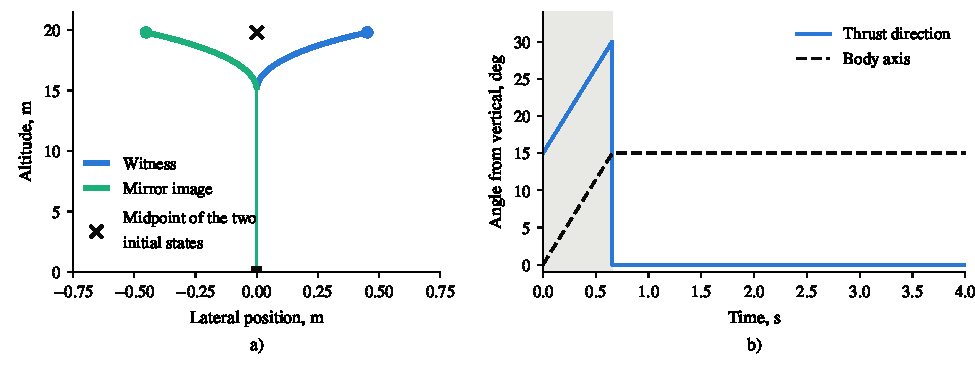
\includegraphics[width=6.5in]{figures/witness.pdf}
\caption{Witnesses of Theorem~\ref{thm:Bstar} for $\Tmin/m_0=5$~m/s$^2$, $\Tmax/m_0=12.5$~m/s$^2$, $\delta=15$~deg,
$\omega=0.4$~rad/s, $s^*=\delta/\omega$, $t_f=4$~s, and constant mass: a)~the two trajectories, with the dive drawn thick and
the lateral scale enlarged; b)~the attitude and thrust direction, with the dive shaded.}\label{fig:witness}
\end{figure}

Figure~\ref{fig:witness} shows the witnesses. With an unlimited rate the body could alternate between the two directions
arbitrarily fast and the midpoint would be landable, which is the 3-DOF situation; with zero rate the thrust could alternate
on the gimbal cone instead. A finite, positive rate limit is what the obstruction needs. The same proof covers upright
touchdown (the body returns to vertical during the brake if $t_f\ge2s^*$), 6-DOF attitude kinematics (the third column of a
rotation matrix with angular velocity bounded by $\omega$ satisfies Eq.~\eqref{eq:AL}), and free final time on a bounded
window, so a search over the final time with a convex program at each value is not lossless either.

\emph{Formal verification.} Theorems~\ref{thm:A} and \ref{thm:Bstar}, both lemmas, and these extensions, with constant
thrust-acceleration bounds and with explicit mass depletion, are formalized in Lean~4 with the Mathlib library
\cite{lean4,mathlib,repo}; the project has no unproved step, and each of the 126 audited declarations depends only on the
three standard axioms. A second reader, working from the manuscript alone, rebuilt the project, wrote an independent
simulator, and searched for a control that lands from $\theta_m$ in the case of Fig.~\ref{fig:witness}; the search came no
closer than 0.020 in the Euclidean norm of $(r_0,v_0)$, whereas it reaches a random landable datum to within $10^{-8}$.
That review also found that an earlier statement of (S1) lacked the bound $\pi/2-\delta$, which the formal statement had
always carried.

\emph{Size of the effect.} Nonconvexity alone does not say how far a complete program must overreach. The proof can be made
quantitative without the equality case: a control whose $W_z$ falls short of $V^*$ by $\eta$ has, by Lemma~\ref{lem:tri}
applied about the body axis at an early instant, nearly the lateral moment of a witness, and tilting during the brake can
cancel that moment only at a cost in $\eta$ that the Cauchy--Schwarz inequality bounds. For $\delta\le\pi/4$ this gives
\begin{equation}\label{eq:eta}
\operatorname{dist}(\theta_m,\F)\ \ge\ \frac{\eta_0}{\sqrt{1+s^{*2}}},\qquad
(1+c_1)\,\eta_0+\sqrt{\tau_{\max}(t_f-s^*)^2\,\eta_0}=\gamma_X:=\frac{5\,\Tmin}{32\,m_0}\sin\delta\,s^{*2},\qquad
c_1=\frac{4\,\tau_{\max}m_0}{\omega\,\Tmin\sin\delta\,s^*} .
\end{equation}
For an 80-kg lander with
thrust between 400 and 1000~N, $\delta=15$~deg, $\omega=0.4$~rad/s, $s^*=\delta/\omega$, and $t_f=7$~s, $\gamma_X=0.087$~m but
$\eta_0=1.3\times10^{-5}$~m: a competitor can cancel the lateral moment of a short dive by tilting slightly during the long
brake. For descents that begin
in the air the gap is therefore proved but small. It grows on short, aggressive maneuvers, as the example of the next
section shows.

%%MODEL%%
\subsection{Status of the Impossibility for This Vehicle}
On the gimbaled rigid body the witnesses of Theorem~\ref{thm:Bstar} are not trajectories, because deflecting the thrust
outward rotates the body inward. Equation~\eqref{eq:cop} turns the problem into one with zero gimbal angle and a bounded
angular acceleration for $y$, and with it we proved nonconvexity of the landing set, with upright touchdown at rest and
$r_z\ge0$, at final times of 1, 2, 3, and 5~s by computer-assisted certificates verified in exact arithmetic \cite{repo}. The
certificates assume constant mass and an unlimited gimbal rate, and the certified distances are between $10^{-6}$ and
$10^{-4}$~m. With a gimbal-rate limit and depleting mass the statement rests on numerical evidence. On the model and planning
limits of Table~\ref{tab:vehicle}, a nonconvex solver \cite{ipopt} finds landings 1, 2, and 3~m from the launch point of a
4-s hop launched straight up at 6.3~m/s, but none on the launch point itself, from symmetric initial guesses or from nine
asymmetric ones (Fig.~\ref{fig:ring}): a vehicle rising too fast for the time allowed must shed vertical impulse, with a minimum throttle it can do
so only by tilting, and tilting carries it sideways. The reachable landing points form a ring, so the landable data are not a
convex set. This is evidence, not a proof of infeasibility.

\begin{figure}[t]\centering
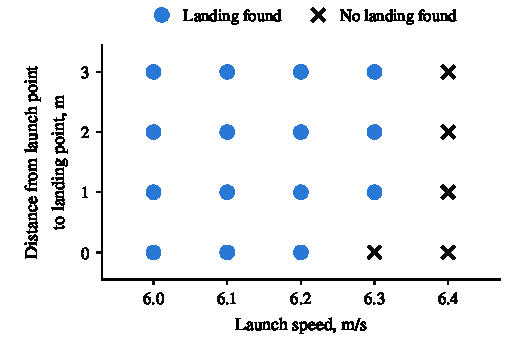
\includegraphics[width=3.4in]{figures/hopring.pdf}
\caption{A 4-s hop of the gimbaled rigid body launched straight up: landing distances at which a nonconvex solver did and did
not find a trajectory.}\label{fig:ring}
\end{figure}

Exactness is therefore out of reach, in proof for the model of Sec.~\ref{sec:problem} and in evidence for this vehicle.
Soundness is not, and Eq.~\eqref{eq:cop} makes it inexpensive.

%%PROGRAM%%
